\documentclass[11pt]{article}
\usepackage{amsmath, amssymb}
\usepackage{geometry}
\usepackage{hyperref}
\usepackage{graphicx}
\usepackage{booktabs}
\geometry{margin=2.5cm}
\graphicspath{{../plots/}}
\emergencystretch=2em

\newcommand{\Pop}{\hat{P}}
\newcommand{\ket}[1]{|#1\rangle}
\newcommand{\dyad}[1]{|#1\rangle\langle#1|}
\newcommand{\Oedge}{X_0 Z_1\cdots Z_{L-2} X_{L-1}}
\newcommand{\expv}[1]{\langle #1\rangle}
\newcommand{\Tr}{\operatorname{Tr}}
\newcommand{\cx}{\texttt{cx}}

\title{Noisy VQE Optimization and Backend-Calibrated Noise\\
\large Removing two idealizations from the Block-4 noise study}
\author{Seminar notes}
\date{\today}

\begin{document}
\maketitle

\begin{abstract}
The Block-4 noise study so far made two convenient assumptions: the variational
state was optimized on a \emph{noiseless} landscape (noise applied only at
evaluation), and the noise itself was a \emph{hand-set uniform} model (one per-\cx{}
depolarizing rate, or one global $T_1/T_2$). This note documents lifting both.
First, we put the noise \emph{inside} the optimizer, so every cost evaluation is a
noisy density-matrix simulation. The finding is a clean dichotomy: for
\textbf{unital} noise (depolarizing) noise-aware optimization changes nothing --
which retroactively \emph{validates} the noiseless-preparation idealization -- while
for \textbf{non-unital} noise (amplitude damping) it raises the \emph{measured} edge
string but \emph{lowers} the noiseless fidelity to the true ground state. Minimizing
the device-level cost is therefore not the same as preparing the state: a better
number can be a worse state. Second, we replace the toy noise with
\texttt{NoiseModel.from\_backend} on a recorded IBM device snapshot
(\texttt{fake\_manila}); the calibrated curve sits \emph{between} the ideal and the
harsh uniform toy, i.e.\ the uniform assumption overstates the damage. Code:
\texttt{src/block4.py}, plots 8 and 9.
\end{abstract}

\section{Setup: what was idealized}

The Block-4 pipeline prepares the even-parity ground state with a
parity-penalized VQE cost
\begin{equation}
  C(\theta) \;=\; \expv{H}_\theta \;+\; \lambda\bigl(1-\expv{\Pop}_\theta\bigr)^2 ,
  \label{eq:cost}
\end{equation}
and then reads the non-local edge string $\expv{\Oedge}$ on the prepared state.
Two idealizations entered:
\begin{enumerate}
  \item \textbf{Noiseless preparation.} $C(\theta)$ was evaluated on the pure
        statevector; the optimizer never saw noise and returned the ideal optimum
        $\theta^\ast$. Noise was applied only afterward, to the fixed $\theta^\ast$.
  \item \textbf{Toy noise.} The channel was a single uniform per-\cx{} depolarizing
        probability $p_{cx}$, or one global thermal $T_1/T_2$ applied identically to
        every qubit.
\end{enumerate}
Sections~\ref{sec:noisy} and~\ref{sec:backend} remove these one at a time.

\section{Noisy VQE optimization}
\label{sec:noisy}

\subsection{Method}

We replace the statevector cost by its noisy counterpart: the transpiled
preparation circuit is run as a density matrix through a Qiskit
\texttt{NoiseModel}, and
\begin{equation}
  C_{\text{noisy}}(\theta)
  = \Tr\!\bigl[H\,\rho_\theta\bigr]
  + \lambda\bigl(1-\Tr[\Pop\,\rho_\theta]\bigr)^2 ,
  \qquad \rho_\theta = \mathcal{E}\bigl(U(\theta)\dyad{0}U^\dagger(\theta)\bigr),
\end{equation}
where $\mathcal{E}$ fires a channel after every \cx{}. Each evaluation is one $4^L$
density-matrix simulation, so the optimizer (COBYLA) is warm-started from the
noiseless optimum $\theta^\ast$ and refined, with a few random restarts; the best
noisy cost is kept. The warm start guarantees the two strategies coincide at zero
noise. Everything is at $L=4$, $r=3$, $\mu=0$ (sweet spot), $\lambda=0.1$.

\subsection{Unital vs.\ non-unital noise}

The two columns of Figure~\ref{fig:noisyvqe} sweep the \emph{same} per-\cx{} error
axis with two channels of opposite character:
\begin{itemize}
  \item \textbf{Depolarizing} is \emph{unital}, $\mathcal{E}(I)=I$: it contracts all
        traceless expectations toward the maximally mixed state without singling out
        a direction. Empirically the noise-aware optimum is indistinguishable from
        $\theta^\ast$ in every observable (Table~\ref{tab:noisy}, top): there is
        nothing for re-optimization to exploit.
  \item \textbf{Amplitude damping} is \emph{non-unital}: it drives every qubit toward
        $\ket{0}$, breaking the symmetry. The energy optimum genuinely moves, and the
        noisy optimizer finds a different $\theta$.
\end{itemize}

\begin{table}[t]
  \centering
  \footnotesize
  \begin{tabular}{lcccc}
    \toprule
    & \multicolumn{2}{c}{noisy $|\expv{\Oedge}|$} & \multicolumn{2}{c}{noiseless fidelity to ED GS}\\
    \cmidrule(lr){2-3}\cmidrule(lr){4-5}
    strength & best-case & noise-aware & best-case & noise-aware\\
    \midrule
    \multicolumn{5}{l}{\emph{Depolarizing (unital), $p_{cx}$:}}\\
    $0.04$ & $0.711$ & $0.712$ & $0.998$ & $1.000$\\
    $0.08$ & $0.502$ & $0.501$ & $0.998$ & $1.000$\\
    $0.12$ & $0.349$ & $0.366$ & $0.998$ & $1.000$\\
    \midrule
    \multicolumn{5}{l}{\emph{Amplitude damping (non-unital), $\gamma$:}}\\
    $0.04$ & $0.656$ & $\mathbf{0.755}$ & $0.998$ & $0.999$\\
    $0.08$ & $0.422$ & $\mathbf{0.565}$ & $0.998$ & $0.994$\\
    $0.12$ & $0.266$ & $\mathbf{0.337}$ & $0.998$ & $\mathbf{0.966}$\\
    \bottomrule
  \end{tabular}
  \caption{Best-case ($\theta^\ast$, noiseless optimum) vs.\ noise-aware (re-optimized
  under the channel), $L=4$, $r=3$, $\mu=0$, $\lambda=0.1$, seed $7$. Under
  depolarizing noise both quantities are unchanged. Under amplitude damping the
  measured edge string \emph{rises} while the noiseless fidelity to the true ground
  state \emph{falls} at strong damping.}
  \label{tab:noisy}
\end{table}

\subsection{The fidelity honesty check}

A lower noisy energy or a higher measured edge string is meaningless if the
underlying state has drifted \emph{away} from the true Majorana ground state -- the
optimizer would then be exploiting the channel rather than preparing the state
better. The decisive quantity is therefore the \textbf{noiseless} fidelity
$|\langle\psi_{\text{ED}}|\psi(\theta)\rangle|^2$ of the re-optimized parameters
(Table~\ref{tab:noisy}, last columns; Figure~\ref{fig:noisyvqe}, bottom row).

The result is unambiguous. At \emph{weak} damping ($\gamma=0.04$) the noise-aware
state keeps essentially the same fidelity ($0.998\!\to\!0.999$) while raising the
edge string -- genuine variational compensation. At \emph{strong} damping
($\gamma\gtrsim0.06$) the edge string still rises, but the noiseless fidelity
\emph{drops} (to $0.94$--$0.97$) and does so non-monotonically and
seed-dependently: the ``recovery'' is partly the optimizer gaming the observable
through the channel, not a better-prepared ground state. So the honest headline is
not ``noise-aware VQE recovers the signal'' but:
\begin{center}
  \emph{minimizing the device-level cost is not the same as preparing the ground
  state.}
\end{center}
Conversely, the unital null is itself a useful result: it shows that for
symmetric gate noise the noiseless-preparation idealization of the rest of Block~4
loses nothing -- the best-case curves are representative, not optimistic.

\begin{figure}[t]
  \centering
  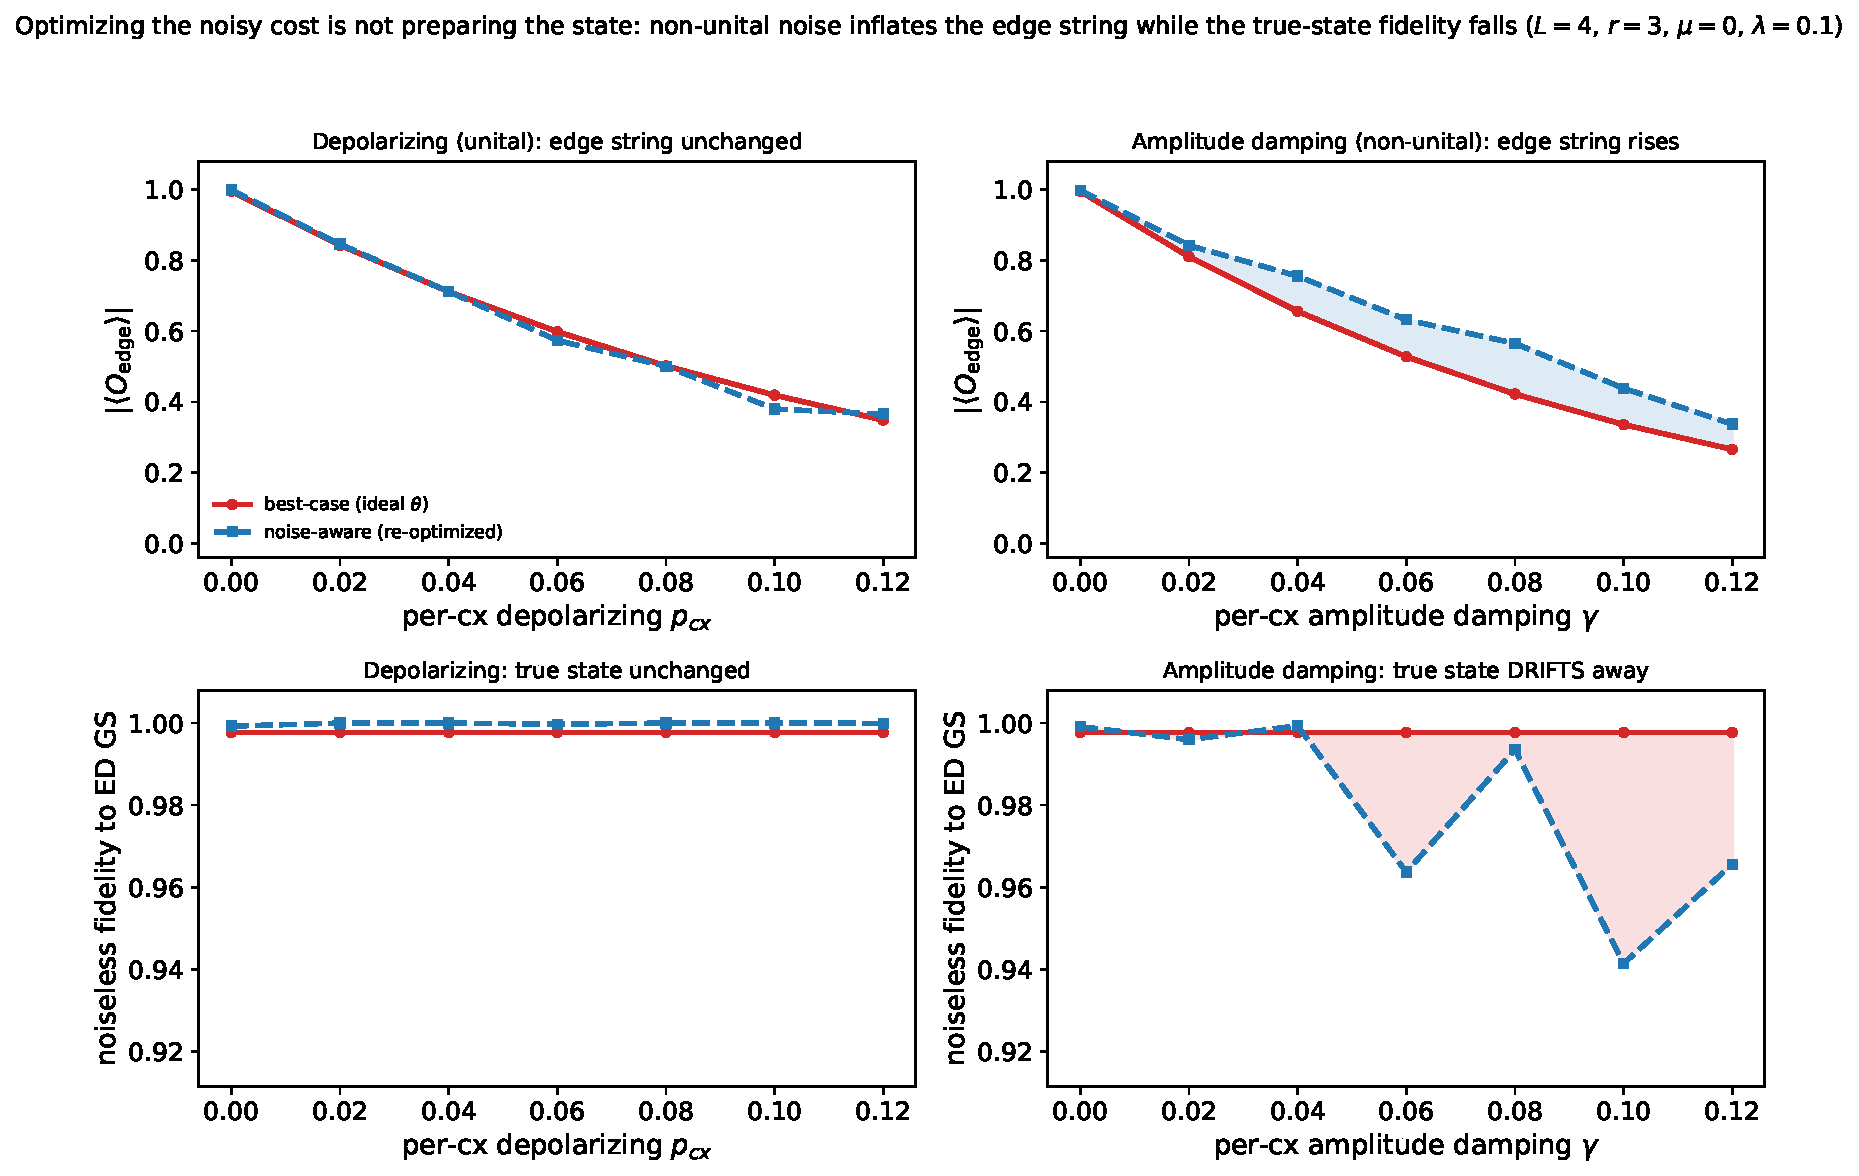
\includegraphics[width=0.92\textwidth]{block4_week9_noisy_vqe.pdf}
  \caption{Best-case vs.\ noise-aware optimization. Columns: depolarizing (unital)
  $\mid$ amplitude damping (non-unital), same per-\cx{} axis. Top: the \emph{measured}
  noisy edge string; bottom: the \emph{noiseless} fidelity to the ED ground state.
  Non-unital noise lets the optimizer inflate the top-row observable while the
  bottom-row fidelity falls.}
  \label{fig:noisyvqe}
\end{figure}

\section{Backend-calibrated noise}
\label{sec:backend}

\subsection{Method}

\texttt{NoiseModel.from\_backend(backend)} builds a channel from a real device's
recorded calibration -- per-qubit $T_1/T_2$, per-\emph{gate} error rates, gate
durations, and readout error -- rather than one hand-set number. We use the IBM
\texttt{fake\_manila} snapshot (a five-qubit linear device shipped with
\texttt{qiskit\_ibm\_runtime}); its \cx{} error rates are heterogeneous,
$\approx0.009$--$0.014$, and its linear coupling matches the chain, so every
nearest-neighbour \cx{} of the ansatz carries a calibrated error. The fixed VQE
angles are then evaluated under this model and compared with the uniform toy on the
identical circuit.

\subsection{Result}

\begin{table}[h]
  \centering
  \footnotesize
  \begin{tabular}{lccc}
    \toprule
    $|\expv{\Oedge}|$ at $\mu=0$ & ideal & backend (\texttt{fake\_manila}) & uniform toy ($p_{cx}=0.05$)\\
    \midrule
    value & $0.99$ & $0.87$ & $0.67$\\
    \bottomrule
  \end{tabular}
  \caption{The calibrated device curve sits between the ideal and the uniform toy.}
  \label{tab:backend}
\end{table}

At the sweet spot the calibrated model costs a meaningful $\sim\!12\%$ of the edge
signal, but far less than the deliberately harsh uniform toy: because the real
per-\cx{} rates ($\sim\!0.01$) are roughly five times smaller than the toy's
$0.05$, a uniform toy model \emph{overstates} the damage
(Table~\ref{tab:backend}, Figure~\ref{fig:backend}). The dominant driver is the
per-gate error \emph{magnitude}; per-qubit heterogeneity is a secondary refinement
at $L=4$.

\subsection{Caveats}

\begin{itemize}
  \item \textbf{Readout error is excluded.} The diagnostic is read as
        $\Tr[\Oedge\,\rho]$ directly from the saved density matrix, with no
        measurement instruction in the circuit. \texttt{from\_backend} does include a
        \texttt{measure} error, but it never fires on this path -- so even the device
        curve is mildly optimistic, since real readout adds $1$--$3\%$ per qubit.
  \item \textbf{Snapshot, not live hardware.} \texttt{fake\_manila} is recorded
        calibration data, representative of the device at snapshot time, not a live
        run. It requires \texttt{qiskit\_ibm\_runtime}; absent that, the code falls
        back to a synthetic \texttt{GenericBackendV2}, whose (seed-generated) error
        rates are much smaller and should \emph{not} be read as a real-device result.
\end{itemize}

\begin{figure}[t]
  \centering
  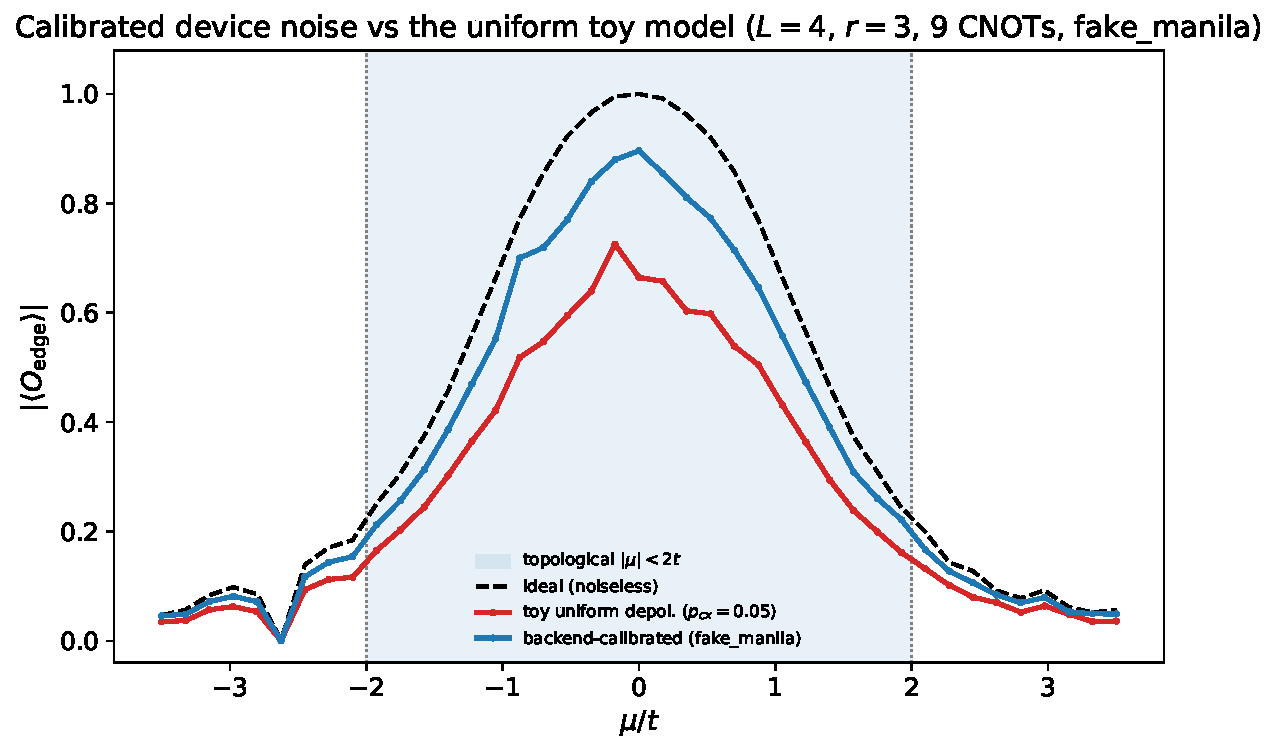
\includegraphics[width=0.7\textwidth]{block4_week9_backend_noise.pdf}
  \caption{Edge string across the phase diagram under ideal, uniform-toy, and
  backend-calibrated (\texttt{fake\_manila}) noise. The calibrated curve lies between
  the other two.}
  \label{fig:backend}
\end{figure}

\section{Takeaways}

\begin{itemize}
  \item Optimizing a noisy cost does not by itself buy a better \emph{state}. For
        symmetric (unital) gate noise it changes nothing; for non-unital noise it can
        raise a chosen observable while degrading fidelity to the target -- an
        artifact to be reported honestly, not a mitigation.
  \item The unital null result is the quiet payoff: it certifies that the
        noiseless-preparation idealization used elsewhere in Block~4 is not hiding an
        optimistic bias for depolarizing noise.
  \item Uniform toy noise is a conservative caricature: a calibrated device model is
        milder, though still not noise-immune, and the device curve here is itself
        optimistic because readout error is excluded.
\end{itemize}

\paragraph{Reproduce.}
\begin{verbatim}
python src/block4.py --plots 8   # noisy VQE optimization (unital vs non-unital)
python src/block4.py --plots 9   # toy vs backend-calibrated noise
\end{verbatim}
Plot~8 uses \texttt{amp\_damp\_noise\_model} / \texttt{noisy\_optimize}; plot~9 uses
\texttt{backend\_noise\_model} (\texttt{NoiseModel.from\_backend}).

\end{document}
